\documentclass{article}

% Language setting
% Replace `english' with e.g. `spanish' to change the document language
\usepackage[english]{babel}

% Set page size and margins
% Replace `letterpaper' with `a4paper' for UK/EU standard size
\usepackage[a4paper,top=2cm,bottom=2cm,left=3cm,right=3cm,marginparwidth=1.75cm]{geometry}

% Useful packages
\usepackage{amsmath}
\usepackage{graphicx}
\usepackage[colorlinks=true, allcolors=blue]{hyperref}
\usepackage{xcolor}
\usepackage{listings}

\colorlet{mygray}{black!30}
\colorlet{mygreen}{green!60!blue}
\colorlet{mymauve}{red!60!blue}

\lstset{
  backgroundcolor=\color{gray!10},  
  basicstyle=\ttfamily,
  columns=fullflexible,
  breakatwhitespace=false,      
  breaklines=true,                
  captionpos=b,                    
  commentstyle=\color{mygreen}, 
  extendedchars=true,              
  frame=single,                   
  keepspaces=true,             
  keywordstyle=\color{blue},      
  language=c++,                 
  numbers=none,                
  numbersep=5pt,                   
  numberstyle=\tiny\color{blue}, 
  rulecolor=\color{mygray},        
  showspaces=false,               
  showtabs=false,                 
  stepnumber=5,                  
  stringstyle=\color{mymauve},    
  tabsize=3,                                     
  title=\lstname 
}


\lstnewenvironment{code}[2][]{%
  \lstset{%
    numbers = left,
    title   = #2,
    #1,
  }%
}{}

\title{Assignment 2.1}
\author{Steinarr Hrafn Höskuldsson}

\usepackage{fancyhdr}
\fancypagestyle{firststyle}
{
   \fancyhf{}
   \fancyhead[L]{Embedded Systems Programming}
   
   \renewcommand{\headrulewidth}{0pt} % removes horizontal header line
}

\newcommand{\mycomment}[1]{}
\begin{document}
\pagestyle{firststyle}
{\let\newpage\relax\maketitle}

\mycomment{
\begin{figure}[h]
    \centering
    \includegraphics[width=0.75\textwidth]{LAB3/Basic1.png}
    \caption{"Switch test" Breadboard set up}
    \label{fig:Switch_test}
\end{figure}

\lstinputlisting[caption=Defining 'ColorMatch' state, label={lst:colormatch}, language=Python, firstline=44, lastline=52]{LAB3/Basic.py}

}

\section*{Part 1}
A new project was created in PlatformIO and a finite state diagram using plantUML was written. 

\lstinputlisting[caption=state.wsd]{Assignment3_1StateBehaviour/docs/diagrams/src/state.wsd}

Which generated the following diagram:
\begin{figure}[h]
    \centering
    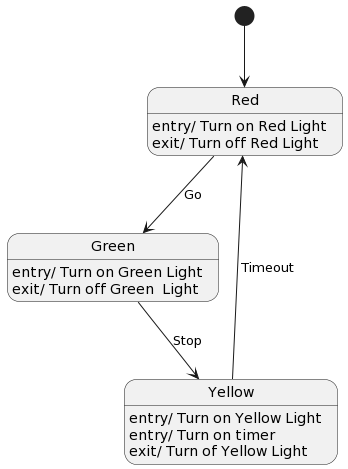
\includegraphics[width=0.5\textwidth]{Assignment3_1StateBehaviour/docs/diagrams/FiniteStateMachine.png}
    \caption{Finite State Machine Diagram of a simplified traffic light.}
    \label{fig:fsmdiagram}
\end{figure}

\section*{Part 2}


\appendix
\section{Code}\label{appendix:code}

\lstinputlisting[caption=timer\_msec.h]{EmbeddedSystemsAssignment2_1/src/timer_msec.h}

\lstinputlisting[caption=timer\_msec.cpp]{EmbeddedSystemsAssignment2_1/src/timer_msec.cpp}

\lstinputlisting[caption=main.cpp]{EmbeddedSystemsAssignment2_1/src/main.cpp}


% TODO: put these in columns next to each other?

\end{document}

